%%%%%%%%%%%%%%%%%%%%%%%%%%%%%%%%%%%%%%%%%%%%%%%%%%%%%%%%%%%%%%%%%%%%%
%                                                                   %
% CHAPTER FIVE: COMPUTATIONAL WALL: LANGFORD PROBLEM                %
%                                                                   %
%%%%%%%%%%%%%%%%%%%%%%%%%%%%%%%%%%%%%%%%%%%%%%%%%%%%%%%%%%%%%%%%%%%%%

\chapter{Computational Wall: Langford Problem}

\section{Introduction}
Our goal is to determine the behavior of accelerators compared to classical processor in case of irregular-computationally heavy problems.
For this purpose we choose the Langford problem which is an academic problem of combinatorial counting.

We present the problem and expose the two possible methods to solve it:
\begin{itemize}[noitemsep,nolistsep]
\item[-] The tree traversal, call Miller's method, providing us benchmark targeting irregular memory and computation. 
\item[-]The algebraic version, calls Godfrey's method, showing the performances of many-core vs multi-core architectures in respect to computationally heavy and memory irregular behaviors.  
\end{itemize}
We show the optimizations made to the regular processor algorithm to efficiently implement this application on GPU. 
We compare the two approaches with classical processor and GPU implementation. 
The results are then presented to show the acceleration using the whole ROMEO supercomputer.
%The Miller's method shows very good results for many-core architecture and the Godfrey's one allows us to beat a world record of computation speed for the two last instances. 

\subsection{The Langford problem}

C. Dudley Langford gave his name to a classic permutation problem ~\cite{Gard56, Simp83}.  
While observing his son manipulating blocks of different colors, he noticed that it was possible to arrange three pairs of different colored blocks (yellow, red and blue) in such a way that only one block separates the red pair - noted as pair 1 - , two blocks separate the blue pair - noted as pair 2 - and finally three blocks separate the yellow one - noted as pair 3 - , see figure~\ref{fig:lang}.\\

\begin{figure}   
\begin{center}    
%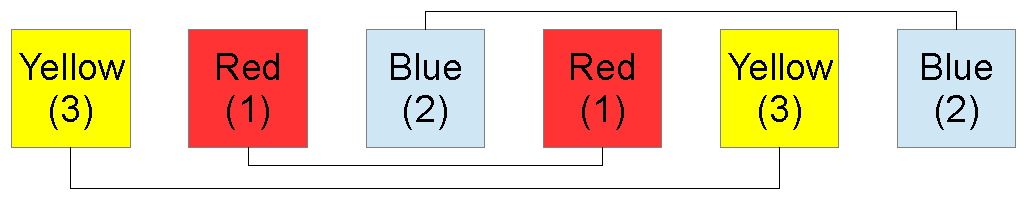
\includegraphics[scale=0.45]{\locpath/figures/langford/lgf_cubes}   
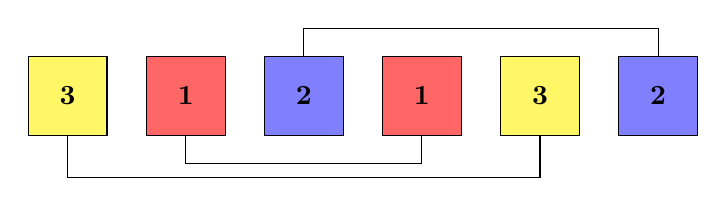
\begin{tikzpicture}
\node (rect) at (0,0) [fill=yellow!60,draw,minimum width=1cm,minimum height=1cm] (p3_1) {\textbf{3}};
\node (rect) at (1.5,0) [fill=red!60,draw,minimum width=1cm,minimum height=1cm] (p1_1) {\textbf{1}};
\node (rect) at (3,0) [fill=blue!50,draw,minimum width=1cm,minimum height=1cm] (p2_1) {\textbf{2}};
\node (rect) at (4.5,0) [fill=red!60,draw,minimum width=1cm,minimum height=1cm] (p1_2) {\textbf{1}};
\node (rect) at (6,0) [fill=yellow!60,draw,minimum width=1cm,minimum height=1cm] (p3_2) {\textbf{3}};
\node (rect) at (7.5,0) [fill=blue!50,draw,minimum width=1cm,minimum height=1cm] (p2_2) {\textbf{2}};
\draw (p3_1.south) -- ([yshift=-15pt]p3_1.south) -- ([yshift=-15pt]p3_2.south) -- (p3_2.south) ;
\draw (p2_1.north) -- ([yshift=10pt]p2_1.north) -- ([yshift=10pt]p2_2.north) -- (p2_2.north) ;
\draw (p1_1.south) -- ([yshift=-10pt]p1_1.south) -- ([yshift=-10pt]p1_2.south) -- (p1_2.south) ;
\end{tikzpicture}  
\end{center}
\caption{L(2,3) arrangement} \label{fig:lang}  
\end{figure}
  
This problem has been generalized to any number $n$ of colors and any number $s$ of blocks having the same color. 
$L(s,n)$ consists in searching for the number of solutions to the Langford problem, up to a symmetry. % ... excepted symmetric ones. 
In November 1967, Martin Gardner presented $L(2,4)$ (two cubes and four colors) as being part of a collection of small mathematical games and he stated that $L(2,n)$ has solutions for all $n$ such that:
\begin{equation}
\text{ solutions for: }
\begin{cases}
n= 4k \\ 
n = 4k-1
\end{cases}
 k \in \mathbb{N}^+
\end{equation}
The central resolution method consists in placing the pairs of cubes, one after the other, on the free places and backtracking if no place is available (see figure~\ref{backtrack} for detailed algorithm).

\begin{table}[t!]
\centering
\[
\begin{tabular}{c r r r}
  \hline
  Instance & Solutions & Method & Computation time\\
  \hline
  \hline
  L(2,3) & 1 &  Miller algorithm & - \\
  L(2,4) & 1 & & - \\ 
  ... & ... & & ...  \\
  L(2,16) & 326,721,800 & & 120 hours  \\
  %\cline{1-3}
  L(2,19) & 256,814,891,280 & & 2.5 years (1999) DEC Alpha \\
  \hline
  \hline
  L(2,20) & 2,636,337,861,200 & Godfrey algorithm & 1 week \\
  %\cline{1-3}
  L(2,23) & 3,799,455,942,515,488 & &  4 days with CONFIIT \\
  %\cline{1-3}
  L(2,24) & 46,845,158,056,515,936 & & 3 months with CONFIIT \\
  L(2,27) & 111,683,611,098,764,903,232 & & 2 days on ROMEO \\
  L(2,28) & 1,607,383,260,609,382,393,152 & & 23 days on ROMEO \\
  \hline
\end{tabular}
\]
\caption{Solutions and time for Langford problem using different methods}
\label{tab:result_base}
\end{table}

The Langford problem has been approached in different ways: discrete mathematics results, specific algorithms, specific encoding, constraint satisfaction problem (CSP), inclusion-exclusion~\ldots~\cite{Mil00,apes-26,Smi00,larsen2009counting}.
In 2004, the last solved instance, $L(2,24)$, was computed by our team \cite{CReSTIC-711} using a specific algorithm. 
Table \ref{tab:result_base} presents the latest results and number of solutions. 
$L(2,27)$ and $L(2,28)$ have just been computed but no details were given. 

The most efficient known algorithms are: the Miller backtrack method, the Godfrey algebraic method and the Larsen inclusion-exclusion method.
The Miller one is based on backtracking and can be modeled as a CSP; it allowed us to move the limit of explicits solutions building up to $L(2,21)$ but combinatorial explosion did not allow us to go further. 
Then, we use the Godfrey method to achieve $L(2,24)$ more quickly and then recompute $L(2,27)$ and $L(2,28)$, presently known as the last instances.
The Larsen method is based on inclusion-exclusion \cite{larsen2009counting}; although this method is effective, practically the Godfrey one is better. 
The latest known work on the Langford Problem is a GPU implementation proposed in \cite{ASS_LGF} in 2015. Unfortunately this study does not provide any performance considerations but just gives the number of solution of $L(2,27)$ and $L(2,28)$.

\section{Miller algorithm}

The Miller's method is based on a tree traversal to be able to check all the cubes positions.
This method finds its limits because even using branch cutting algorithm to traverse the tree, the number of branches to explore stay very high. 
We implemented a multi-core and many-core version of it for the purpose of our benchmark. 
Indeed, this huge tree traversal requires irregular computation and memory accesses: two elements fitting the wall we want to confront to our architectures. 

In this section we present our multi-GPU cluster implementation of the Miller's algorithm. 
First, we introduce the backtrack method itself and the elements allowing us to consider it as a good candidate for our metric. 
Then we present our implementation in order to fit the GPUs architecture. 
The last section presents our results. 

\subsection{CSP}

Combinatorial problems are NP-complete \cite{GJ79} and can be described as satisfiability problems\index{SAT problem} (SAT) using a polynomial transformation. 
They can be transformed into CSP formalism.
A \textit{Constraint Satisfaction Problem}\index{Constraint Satisfaction Problem} (CSP), first introduced by Montanari \cite{Mon74}, is defined as a triple $<X,D,C>$ where:
\begin{equation}
\begin{cases}
X=\{X_1,...,X_n\}\text{: a finite set of variables} \\ 
D=\{D_1,...,D_n\}\text{: their finite domains of values}\\
C=\{C_1,...,C_p\}\text{: a finite set of constraints}
\end{cases}
\end{equation}

The goal in this formalism is to assign values in $D$ to $n$-uple $X$ respecting all the $C$ $p$-uple constraints.
This approach is a large field of research. \cite{arbelaez2014gpu} developed \textit{local search} and compares GPU to CPU. 
This first work brings to light that GPU is a real contributor to the global computation speed. \cite{campeotto2014exploring} proposes a solver using \textit{propagator} on a GPU architecture to solve CSP problems. 
\cite{jenkins2011lessons} cares about GPU weak points, loading bandwidth and global memory latency.

%\subsection{CSP parallel resolution}
%\label{sec:CSP_resolution}

Considering a basic approach, combinatorial problems formed into CSP can be represented as a tree search. Each level corresponds to a given variable, with values in its domain. Leaves of the tree correspond to a complete assignment (all variables are set). If it meets all the constraints this assignment is called an acceptor state. Depending on the constraints set, the satisfiability evaluation can be made either on complete or partial assignment.
%
%There are many ways to browse the tree and find the solutions: \emph{backtracking}, \emph{forward-checking}, \emph{backjumping}, etc. 
%We limit our method to the naive \emph{backtrack} resolution. We chose to evaluate the variables and their values in a static order; in a depth-first manner, the solution is built incrementally and if a partial assignment can be aborted, the branch is cut. A solution is found each time a leaf is reached.
%% presents a backtrack search with the previous CSP representation.
%
%The recommendation for performance on GPU accelerator is to use non test-based programs.
%Due to its irregularity, the basic \emph{backtracking} algorithm is suppose not to suit the GPU architecture.
%Thus a vectorized version is given when evaluating the assignments at the leaves' level, with one of the two following ways: assignments can be prepared on each tree node or totally set on final leaves before testing the satisfiability of the built solution, Fig.\ref{fig:algos}.
%
%\begin{figure}[htbf]
%\begin{minipage}[b]{0.45\linewidth}
%\begin{verbatim}
%for variable_1 
%   assignment
%   for variable_2
%      assignment
%      ...
%         for variable_n
%            assignment
%            test
%\end{verbatim}
%\end{minipage}
%\begin{minipage}[b]{0.45\linewidth}
%\begin{verbatim}
%for variable_1 
%   for variable_2
%   ...
%      for variable_n
%         assignments
%         test
%         
%         
%\end{verbatim}
%\end{minipage} 
%\caption{CSP regularized algorithms}
%\label{fig:algos}
%\end{figure} 
%
%With this method it is necessary to browse the entire tree but this requires using all the search space and it is too time-consuming.
%
%In order to overcome this we divide the work between CPU and GPU. The CPU generates some levels of the tree and creates tasks. Then GPU and CPU cores divide up the workload in order to achieve the generation on the latest levels of the tree. With this method, inconsistent branches can be cut on highest level and GPU/CPU cores only compute possibly consistent tasks.
%
%This representation enables a server-client model to distribute the tasks: the server generates independent sub-problems at a chosen depth in the tree, treated by clients. 
%Each client decomposes the sub-problem into tasks, distributed over the GPU/CPU cores, Fig.\ref{fig:parallel}.
%
%\begin{figure}[htbf]
%\centering 
%\includegraphics[scale=0.9]{figures/graphe_repartition}   
%\caption{Server client distribution} \label{fig:parallel}    
%\end{figure} 
%
%With this method numerous branches have been cut from the main tree during generation stage and GPU/CPU tasks are faster due to their lower depth. Despite the combinatorial explosion of this kind of problem, we can consider solving CSP in a massively parallel manner on multiGPU clusters.

\subsection{Backtrack resolution}

As presented above the Langford problem is known to be a highly irregular combinatorial problem. 
We first present here the general tree representation and the ways we regularize the computation for GPUs.
Then we show how to parallelize the resolution over a multi-GPU cluster.

\subsubsection{Langford's problem tree representation}
\label{sec:LGF_resolution}
%In~\cite{HKS02}, we propose to formalize the Langford problem as a CSP  ({\it Constraint Satisfaction Problem}), first introduced by Montanari in \cite{Mon74}, and show that an efficient parallel resolution is possible. 
As explained, CSP formalized problems can be transformed into tree evaluations. %represented as trees. 
%The tree Here we intend to develop a specific algorithm taking into account the conclusion of our previous studies (memory management of memory and load balance) and transfer the tasks resolution into GPUs.\\
%\begin{figure}[htb]
%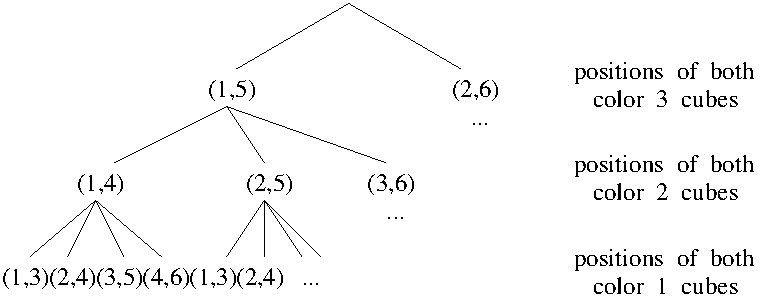
\includegraphics[scale=.65]{\locpath/figures/langford/arbre_en}
%\end{figure}
\begin{figure}[t!]
\centering
\resizebox {\columnwidth} {!} {
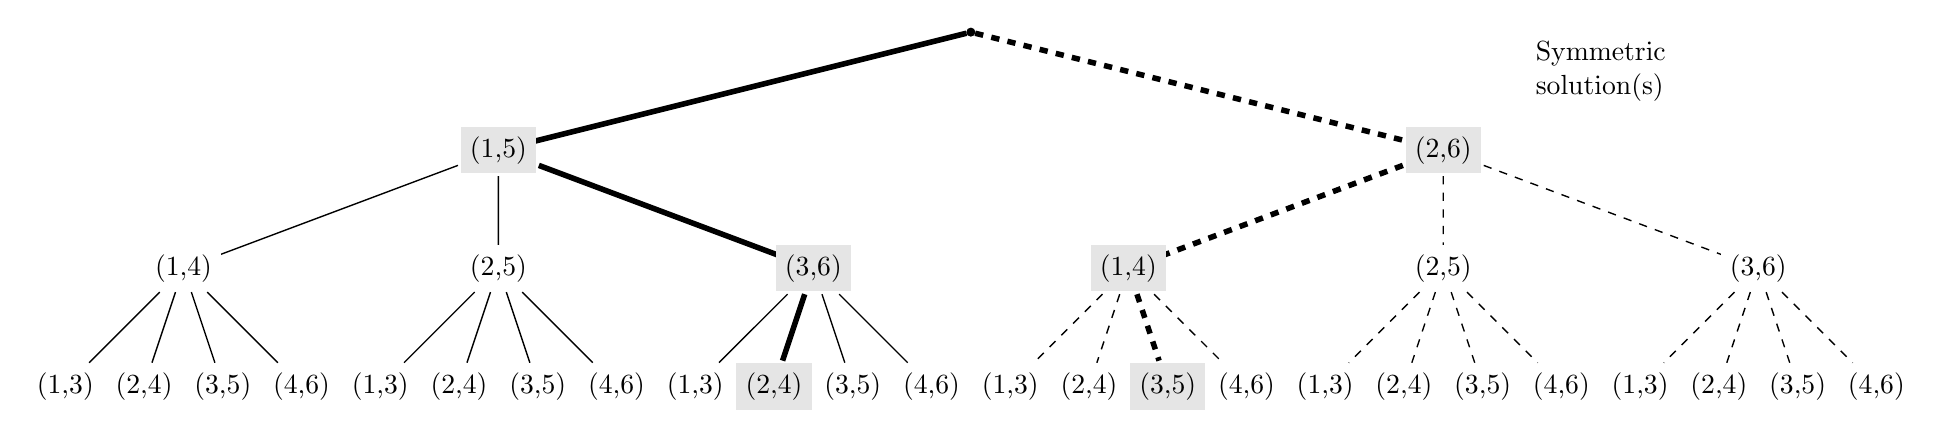
\begin{tikzpicture}[sibling distance=12cm]
%\node at (-13.5,-1.5) {pair 3 positions};
%\node at (-13.5,-3) {pair 2 positions};
%\node at (-13.5,-4.5) {pair 1 positions};
\node [align=left] at (8,-.5) {Symmetric\\solution(s)};
\node  [circle,draw,fill,inner sep=1] {}
  child [line width=2pt] { [sibling distance=4cm] node [fill=black!10] {(1,5)}
    child [line width=.5pt] { [sibling distance=10mm] node [fill=white] {(1,4)}
      child {node {(1,3)}}
      child {node {(2,4)}}
      child {node {(3,5)}}
      child {node {(4,6)}}
    }
    child [line width=.5pt] { [sibling distance=10mm] node [fill=white] {(2,5)}
      child {node {(1,3)}}
      child {node {(2,4)}}
      child {node {(3,5)}}
      child {node {(4,6)}}
    }
    child { [sibling distance=10mm] node [fill=black!10] {(3,6)}
      child [line width=.5pt] {node {(1,3)}}
      child {node [fill=black!10] {(2,4)}}
      child [line width=.5pt] {node {(3,5)}}
      child [line width=.5pt] {node {(4,6)}}
    }
  }
  child [dashed,line width=2pt] { [sibling distance=4cm] node [fill=black!10] {(2,6)}
    child { [sibling distance=10mm] node [fill=black!10] {(1,4)}
      child [line width=.5pt] {node {(1,3)}}
      child [line width=.5pt] {node {(2,4)}}
      child {node [fill=black!10] {(3,5)}}
      child [line width=.5pt] {node {(4,6)}}
    }
    child [line width=.5pt] { [sibling distance=10mm] node [fill=white] {(2,5)}
      child {node {(1,3)}}
      child {node {(2,4)}}
      child {node {(3,5)}}
      child {node {(4,6)}}
    }
    child [line width=.5pt] { [sibling distance=10mm] node [fill=white] {(3,6)}
      child {node {(1,3)}}
      child {node {(2,4)}}
      child {node {(3,5)}}
      child {node {(4,6)}}
    }
  }
;
\end{tikzpicture}
}
\caption{Search tree for $L(2,3)$}
\label{fig:arbre}
\end{figure}
In order to solve $L(2,n)$, we consider a tree of height $n$: see example of $L(2,3)$ in figure~\ref{fig:arbre}.

\begin{itemize}   
\item[-] Every level of the tree corresponds to a cube color.
\item[-] Each node of the tree corresponds to the placement of a pair of cubes without worrying about the other colors. Color $p$ is represented at depth $n-p+1$, where the first node corresponds to the first possible placement (positions 1 and $p+2$) and $i^{th}$ node corresponds to the placement of the first cube of color $p$ in position $i, \ i \in [1, \ 2n-1-p]$.
\item[-] Solutions are leaves generated without any placement conflict.
\item[-] As we consider the solution up to a symmetry, the left part is represented dashed and is in fact not traversed.
\end{itemize}

There are many ways to browse the tree and find the solutions: \emph{backtracking}, \emph{forward-checking}, \emph{backjumping}, etc \cite{prosser93hybrid}. 
We limit our study to the naive \emph{backtrack} resolution and choose to evaluate the variables and their values in a static order; in a depth-first manner, the solutions are built incrementally and if a partial assignment can be aborted, the branch is cut. A solution is found each time a leaf is reached.
% presents a backtrack search with the previous CSP representation.

The recommendation for performance on GPU accelerators is to use non test-based programs.
Due to its irregularity, the basic \emph{backtracking} algorithm, presented on figure~\ref{backtrack}, is not supposed to suit the GPU architecture.
Thus a vectorized version is given when evaluating the assignments at the leaves' level, with one of the two following ways: assignments can be prepared on each tree node or totally set on final leaves before testing the satisfiability of the built solution (figure~\ref{regularized}).

\begin{figure}[t!]
\begin{minipage}[b]{0.45\linewidth}
\footnotesize
\begin{verbatim}
while not done do
 test pair            <- test
 if successful then 
   if max depth then
     count solution
     higher pair	                  
   else
     lower pair       <- remove
 else
   higher pair        <- add
\end{verbatim}
\caption{Backtrack algorithm}\label{backtrack}
\end{minipage}
\begin{minipage}[b]{0.45\linewidth}
\footnotesize
\begin{verbatim}
for pair 1 positions
  assignment                   <- add
  for pair 2 positions
    assignment                 <- add
    for ...
      for pair n positions
        assignment             <- add
        if final test ok then  
          count solution
\end{verbatim}
\caption{Regularized algorithm}\label{regularized}
\end{minipage}
\end{figure}

\subsubsection{Data representation}

\begin{figure}[t!]
\begin{minipage}[b]{0.40\linewidth}
\centering
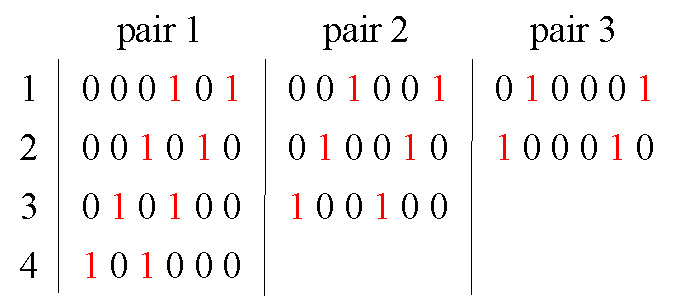
\includegraphics[width=\columnwidth]{\locpath/figures/langford/positions_lgf}
\caption{ Bitwise representation of pairs positions in $L(2,3)$} \label{fig:comb1}
\end{minipage}
\hfill
\begin{minipage}[b]{0.55\linewidth}
\centering
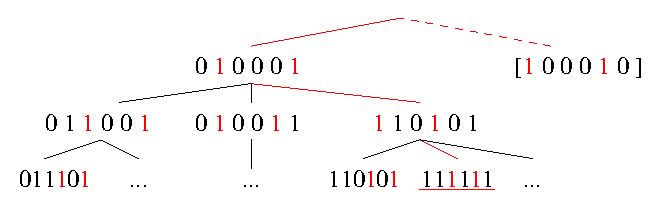
\includegraphics[width=\columnwidth]{\locpath/figures/langford/pos_lgf_v2}
\caption{Bitwise representation of the Langford $L(2,3)$ placement tree}\label{fig:pos_lgf}
\end{minipage}
\end{figure}

In order to count every Langford problem solution, we first identify all possible combinations for one color without worrying about the other ones. 
Each possible combination is coded within an integer, a bit to 1 corresponding to a cube presence, a 0 to its absence. This is what we called a \emph{mask}.
This way figure~\ref{fig:comb1} presents the possible combinations to place the one, two and three weight cubes for the $L(2,3)$ Langford instance.

Furthermore the masks can be used to evaluate the partial placements of a chosen set of colors: all the 1 correspond to occupied positions; the assignment is consistent \emph{iff} there are as many 1 as the number of cubes set for the assignment. 

With the aim to find solutions, we just have to go all over the tree and \emph{sum} one combination of each of the colors: a solution is found \emph{iff} all the bits of the sum are set to 1. 

Each route on the tree can be evaluated individually and independently; then it can be evaluated as a thread on the GPU.
This way the problem is massively parallel and can be, indeed, computed on GPU. figure~\ref{fig:pos_lgf} represents the tree masks' representation.

\subsubsection{Specific operations and algorithms}

Three main operations are required in order to perform the tree search. 
%The first one, allowing to check if a pair can be added to a given partial assignment, is only necessary for the original backtrack scheme.
%The second one, used for both backtrack and regularized methods, aims to add a pair to a given assignment. 
The first one, used for both backtrack and regularized methods, aims to add a pair to a given assignment. 
The second one, allowing to check if a pair can be added to a given partial assignment, is only necessary for the original backtrack scheme.
The last one is used for testing if a global assignment is an available solution: it is involved in the regularized version of the Miller algorithm.

\begin{figure}[t!]
\begin{minipage}[b]{0.5\linewidth}
\centering
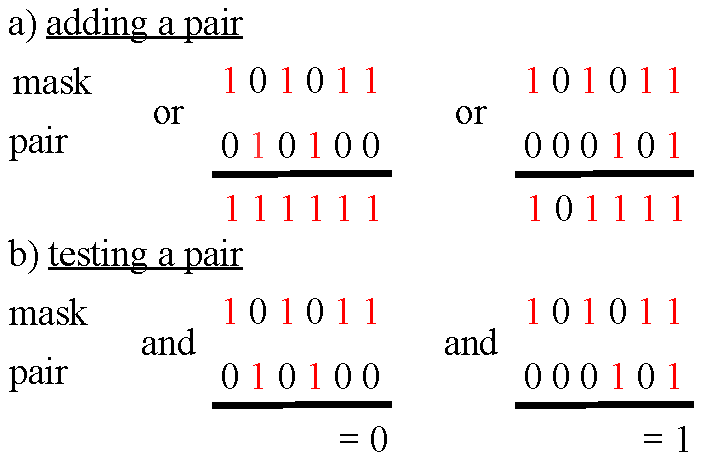
\includegraphics[scale=.5]{\locpath/figures/langford/test_gen}
\caption{Testing and adding position} \label{fig:test_et}
\end{minipage}
\begin{minipage}[b]{0.5\linewidth}
\centering 
\includegraphics[scale=.75]{\locpath/figures/langford/graphe_repartition}   
\caption{Server client distribution} \label{fig:parallel} 
\end{minipage}
\end{figure}

\paragraph{Add a pair: }
Top of figure~\ref{fig:test_et} presents the way to add a pair to a given assignment.
With a \emph{binary OR}, the new mask contains the combination of the original mask and of the added pair.
This operation can be performed even if the position is not available for the pair (however the resulting mask is inconsistent). 

\paragraph{Test a pair position: }
On the bottom part of the same figure, we test the positioning of a pair on a given mask. 
For this, it is necessary to perform a \emph{binary AND} between the mask and the pair.
\begin{itemize}
	\item[] $=0$: \emph{success}, the pair can be placed here
	\item[] $\neq0$: \emph{error}, try another position
\end{itemize}

\paragraph{Final validity test: }
The last operation is for \emph{a posteriori} checking. For example the mask $101111$, corresponding to a leaf of the tree, is inconsistent and should not be counted among the solutions.
The final placement mask corresponds to a solution \emph{iff} all the places are occupied, which can be tested as $\neg mask = 0$. % \rightarrow solution$ else $inconsistent$.
%We performed a \emph{binary not} on the mask. If there is a zero, so the mask is inconsistent, result will be different of zero. If the mask is full of $1$, result is zero, so we can add one to the number of solutions.
\\

Using this data representation, 
we implemented both \emph{backtrack} and \emph{regularized} versions of the Miller algorithm, as presented in figure~\ref{backtrack} and \ref{regularized}.
% C'est là que je veux changer la structure ....
%: the original backtrack for CPU computation and the regularized one for GPUs.
%As we have seen above, the regularized algorithm is unsuitable due to combinatorial explosion, that is why we use the hybrid method on a distributed architecture.
\\
The next section presents the way we hybridize these two schemes in order to get an efficient parallel implementation of the Miller algorithm.

%%%%%%%%%%%%%%%%%%%%%%%%%%%%%%%%%%%%%%%%
\subsection{Hybrid parallel implementation}
\label{section:parallel_backtrack}
Section \ref{sec:LGF_resolution} presents the Miller algorithm and the tools needed for the resolution. 
The irregularity is present in the tree traversal and specific data representation has been chosen for efficient use of the memory. 
This section presents our methodology to implement Miller's method on a multi-GPU cluster.

\paragraph{Tasks generation: }
In order to parallelize the resolution we have to generate tasks. 
Considering the tree representation, we construct tasks by fixing the different values of a first set of variables [pairs] up to a given level. Choosing the development level allows to generate as many tasks as necessary. This leads to a \textit{Finite number of Irregular and Independent Tasks} (\emph{FIIT} applications \cite{krajecki1999object}). 

\paragraph{Cluster parallelization: } 
The generated tasks are independent and we spread them in a client-server manner: a server generates them and makes them available for clients. As we consider the cluster as a set of CPU-GPU(s) machines, the clients are these machines. 
At the machines level, the role of the CPU is, first, to generate work for the GPU(s): it has to generate sub-tasks, by continuing the tree development as if it were a second-level server, and the GPU(s) can be considered as second-level client(s). \\
The sub-tasks generation, at the CPU level, can be made in parallel by the CPU cores. Depending on the GPUs number and their computation power the sub-tasks generation rhythm may be adapted, to maintain a regular workload both for the CPU cores and GPU threads: some CPU cores, not involved in the sub-tasks generation, could be made available for sub-tasks computing.\\
This leads to the 3-level parallelism scheme presented in figure~\ref{fig:parallel}, where $p$, $q$ and $r$ respectively correspond to: ($p$) the server-level tasks generation depth, ($q$) the client-level sub-tasks generation one, ($r$) the remaining depth in the tree evaluation, \textit{i.e.} the number of remaining variables to be set before reaching the leaves.  

\paragraph{\emph{Backtrack} and \emph{regularized} methods hybridization: } 
The Backtrack version of the Miller algorithm suits CPU execution and allows to cut branches during the tree evaluation, reducing the search space and limiting the combinatorial explosion effects. A regularized version had to be developed, since GPUs execution requires synchronous execution of the threads, with as few branching divergence as possible; however this method imposes to browse the entire search space and is too time-consuming. \\
We propose to hybridize the two methods in order to take advantage of both of them for the multiGPU parallel execution: 
for tasks and sub-tasks generated at sever and client levels, the tree development by the CPU cores is made using the backtrack method, cutting branches as soon as possible [and generating only possible tasks]; when computing the sub-tasks generated at client-level, the CPU cores involved in the sub-tasks resolution use the backtrack method and the GPU threads the regularized one. 

%With this method it is necessary to browse the entire tree but this requires using all the search space and it is too time-consuming.

%In order to overcome this we divide the work between CPU and GPU. The CPU generates some levels of the tree and creates tasks. Then GPU and CPU cores divide up the workload in order to achieve the generation on the latest levels of the tree. 
%With this method, inconsistent branches can be cut on highest level and GPU/CPU cores only compute possibly consistent tasks.

%This representation enables a server-client model to distribute the tasks: the server generates independent sub-problems at a chosen depth in the tree, treated by clients. 
%Each client decomposes the sub-problem into tasks, distributed over the GPU/CPU cores, Fig.~\ref{fig:parallel}.

%By doing so numerous branches have been cut from the main tree during generation stage and GPU/CPU tasks are faster due to their lower depth. Despite the combinatorial explosion of this kind of problem, we can consider solve it in a massively parallel manner on multiGPU clusters.
 
%The tree representation allows to generate tasks at a chosen level, which leads to a \textit{Finite number of Irregular and Independent Tasks} (\emph{FIIT} applications \cite{krajecki1999object}).
%We set up a server-client distribution. The server, client and GPU parts have their own development depth, respectively $p$, $q$ and $r$, $p+q+r=n$, Fig.~\ref{fig:parallel}.
%\begin{itemize}
%\item \texttt{Server} generates sub-problems by placing $p$ pairs on masks with the $backtrack$ algorithm.
%\item \texttt{Client} starts with a mask generated by the server and produces tasks by adding $q$ pairs in the initial mask, with the $backtrack$ algorithm. Then the client creates specific tasks by pre-computing the available positions for placing pairs. For example with the $10100110$ mask the second pair can be placed on only two positions, $01001000$ and $00001001$, that match positions 2-5 and 5-8. Instead of browsing all the 5 positions and test, the GPU just has to try 2 positions for this pair. Thus we greatly reduce the GPU load computation.
%\item \texttt{CPUs and GPUs} can compute in competition. Whereas CPUs use standard backtrack, GPUs generate leaves using the regularized method and adding successive pairs on their masks without any test.  
%\end{itemize}

\subsection{Experiments tuning}

In order to take advantage of all the computing power of the GPU we have to refine the way we use them: this section presents the experimental study required to choose optimal settings. This tuning allowed us to prove our proposal on significant instances of the Langford problem.

\paragraph{Registers, blocks and grid: }

In order to use all GPUs capabilities, the first way was to fill the blocks and grid. To maximize occupancy (ratio between active warps and the total number of warps) NVIDIA suggests to use 1024 threads per block to improve GPU performances and proposes a CUDA occupancy calculator\footnote{\url{http://developer.download.nvidia.com/compute/cuda/CUDA_Occupancy_calculator.xls}}. But, confirmed by the Volkov's results\cite{Volkov}, we experimented that better performances may be obtained using lower occupancy. Indeed, another critical criterion is the inner GPU registers occupation. 
The optimal number of registers ($57$ registers) is obtained by setting 9 pairs placed on the client for $L(2,15)$, thus 6 pairs are remaining for GPU computation.

\begin{figure}[t!]
\centering
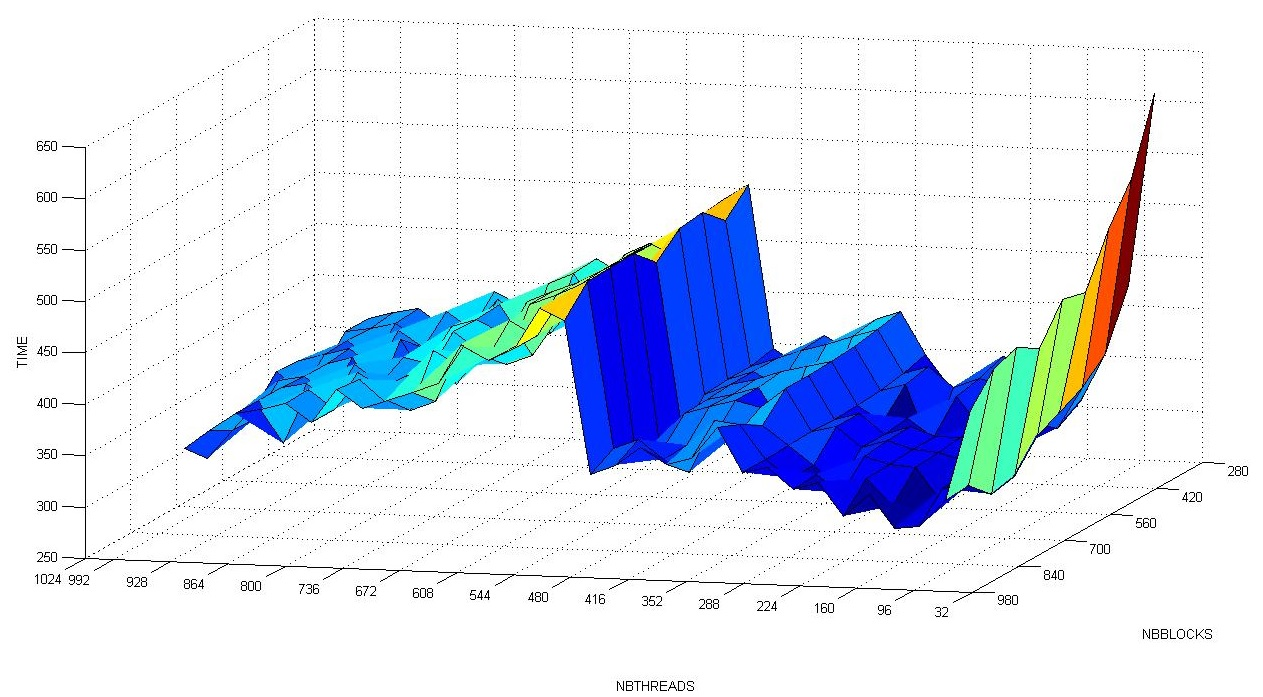
\includegraphics[scale=.4]{\locpath/figures/langford/graphe_15_9}
\caption{Time depending on grid and block size on $n=15$}
\label{f7}
\end{figure}

In order to tune the blocks and grid sizes, we performed tests on the ROMEO architecture. 
%0 With this value we obtained an optimized number of registers by thread . 
Figure~\ref{f7} represents the time in relation with the number of blocks per grid and the number of threads per block. 
The most relevant result, observed as a local minimum on the 3D surface, is obtained near 64 or 96 threads per block; for the grid size, the limitation is relative to the GPU global memory size.
It can be noted that we do not need shared memory because their are no data exchanges between threads. 
This allows us to use the total available memory for the L1 cache for each thread.

\paragraph{Streams:}
A client has to prepare work for GPU. There are four main steps: generate the tasks, load them into the device memory, process the task on the GPU and then get the results.

\begin{figure}[t!]
\begin{minipage}[b]{0.48\linewidth}
\centering
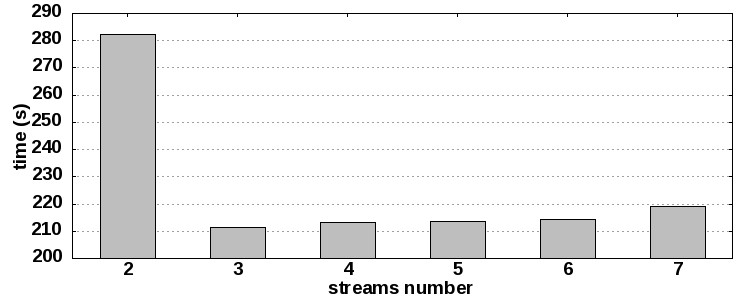
\includegraphics[width=\columnwidth]{\locpath/figures/langford/streams.jpeg}
\caption{Computing time depending on streams number}
\label{fig:streams}
\end{minipage}
\hfill
\begin{minipage}[b]{0.48\linewidth}
\centering
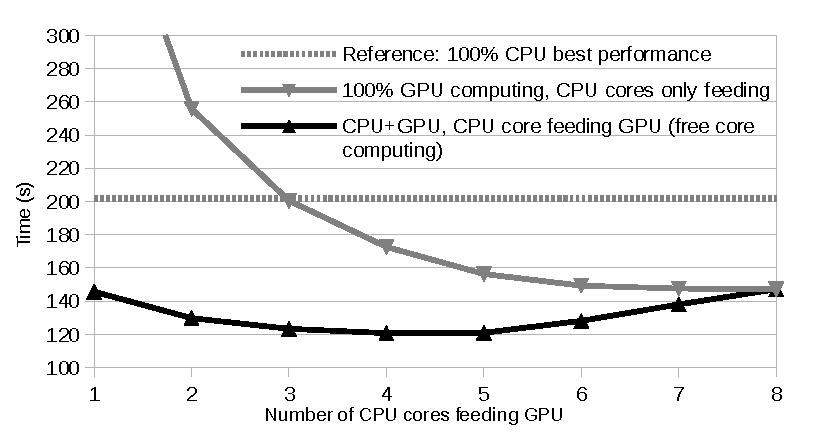
\includegraphics[width=\columnwidth]{\locpath/figures/langford/graphe_cores.pdf}
\caption{CPU cores optimal distribution for GPU feeding}\label{cores_rep}
\end{minipage}
\end{figure}

CPU-GPU memory transfers cause huge time penalties (about 400 cycles latency for transfers between CPU memory and GPU \emph{device memory}). 
At first, we had no overlapping between memory transfer and kernel computation because the tasks generation on CPU was too long compared to the kernel computation.
To reduce the tasks generation time we used OpenMP in order to use the eight available CPU cores.
Thus CPU computation was totally hidden by memory transfers and GPU kernel computation. We tried using up to 7 streams; as shown by figure~\ref{fig:streams}, using only two simultaneous streams did not improve efficiency because the four steps did not overlap completely; the best performances were obtained with three streams; the slow increase in the next values is caused by synchronization overhead and CUDA streams management.

\paragraph{Setting up the server, client and GPU depths: }
We now have to set the depths of each actor, server $(p)$, client $(q)$ and GPU $(r)$ (see figure~\ref{fig:parallel}).

First we set the $r = 5$ for large instances because of the GPU limitation in terms of registers by threads, exacerbated by the use of numerous $64bits$ integers. For $r \geq 6$, we get too many registers (64) and for $r \leq 4$ the GPU computation is too fast compared to the memory load overhead.

Clients are the buffers between the server and the GPUs: 
$q = n - p- r$.
So we have conducted tests by varying the server depth, $p$. The best result is obtained for $p=3$ and performance decreases quickly for higher values. This can be explained since more levels on the server generates smaller tasks; thus GPU use is not long enough to overlap memory exchanges.
% because with more levels on the server, tasks are smaller and then the GPU work is not long enough in view of memory exchanges.

\paragraph{CPU: Feed the GPUs and compute}
The first work of CPU cores is to prepare tasks for GPU so that we can generate overlapping between memory load and kernel computation. 
In this configuration using eight cores to generate GPU tasks under-uses CPU computation power. 
It is the reason why we propose to use some of the CPU cores to take part of the sub-problems treatment. 
Figure~\ref{cores_rep} represents computation time in relation with different task distributions between CPU and GPU.
We experimentally demonstrated that only 4 or 5 CPU cores are enough to feed GPU, the other ones can be used to perform backtrack resolution in competition with GPUs.

\subsection{Results}

\paragraph{Regularized method results}
We now show the results obtained for our massively parallel scheme using the previous optimizations, comparing the computation times of successive instances of the Langford problem. 
These tests were performed on 20 nodes of the ROMEO supercomputer, hence 40 CPU/GPU machines.

The previous limit with Miller's algorithm was $L(2,19)$, obtained in 1999 after 2.5 years of sequential effort and at the same time after 2 months with a distributed approach\cite{Mil00}. 
Our computation scheme allowed us to obtain it in less than 4 hours (Table \ref{tab:result_base_regu}), this being not only due to Moore law progress.\\
Note that the computation is 1.6 faster with CPU+GPU together than using 8 CPU cores. 
In addition, the GPUs compute $200,000\times$ more nodes of the search tree than the CPUs, with a faster time.

\begin{table}[t!]
\begin{subfigure}[b]{0.5\linewidth}
\centering
\begin{tabular}{l r r r}
					\hline
					$n$ & CPU (8c) &  GPU (4c) +  &  \hspace*{-.8em}CPU (4c) \\
					\hline
					\hline
					15	& 2.5 & 1.5 & \\
					16  & 21.2 &14.3 & \\
					17  & 200.3 &120.5 &\\
					18  & 1971.0 &1178.2 &\\
					19  & 22594.2 & 13960.8 & \\ 
					\hline
\end{tabular}
\caption{Regularized method (seconds)}
\label{tab:result_base_regu}
\end{subfigure}
\begin{subfigure}[b]{0.5\linewidth}
\centering
\begin{tabular}{ l r r r }
					\hline
					$n$ & CPU (8c) &  GPU (4c) +  &  \hspace*{-.8em}CPU (4c) \\
					\hline
					\hline
					17  & 29.8 & 7.3&\\
					18  & 290.0 & 73.6&\\
					19  & 3197.5 & 803.5& \\
					20  & -- & 9436.9 &\\
					21  & -- & 118512.4& \\ 
					\hline
\end{tabular}	
\caption{Backtrack  (seconds)}
\label{tab:result_backtrack}
\end{subfigure}
\caption{Comparison between multi-core processors and GPUs for regularized and backtrack method}
\end{table}

The computation time between two different consecutive instances being multiplied by $10$ approximately, this could allow us to obtain $L(2,20)$ in a reasonable time.


\paragraph{Backtracking on GPUs}

It appears at first sight that using backtracking on GPUs without any regularization is a bad idea due to threads synchronization issues.
But in order to compare CPU and GPU computation power in the same conditions we decided to implement the original backtrack method on GPU (see figure~\ref{backtrack}) with only minor modifications.
In these conditions we observe very efficient work of the NVIDIA scheduler, which perfectly handles threads de-synchronization.
Thus we use the same server-client distribution as in \ref{section:parallel_backtrack}, each client generates masks for both CPU and GPU cores. 
The workload is then statically distributed on GPU and CPU cores.
Executing the backtrack algorithm on a randomly chosen set of sub-problems allowed us to set the GPU/CPU distribution ratio experimentally to 80/20\%.

The experiments were performed on 129 nodes of the ROMEO supercomputer, hence 258 CPU/GPU machines and one node for the server. 
Table \ref{tab:result_backtrack} shows the results with this configuration. 
This method first allowed us to perform the computation of $L(2,19)$ in less than 15 minutes, $15\times$ faster than with the regularized method; then, we pushed the limitations of the Miller algorithm up to $L(2,20)$ in less than 3 hours and even $L(2,21)$ in about $33$ hours\footnote{Even if this instance has no interest since it is known to have no solution}.\\

This first benchmark application provides a perfect example for the behavior of many-core accelerators confronted to irregular application.
Even if the application does not seemed to fit with the direct tree traversal, the results prove that if used in the right way performance can be achieve in this case. 


%%%%%%%%%%%%%%%%%%%%%%%%%%%%%%%%%%%%%%%
%                                     %
%                                     %
% GODFREY                             %
%                                     %
%                                     %
%%%%%%%%%%%%%%%%%%%%%%%%%%%%%%%%%%%%%%%

\section{Godfrey's algebraic method}
The previous part presents the Miller algorithm for the Langford problem, this method cannot achieve bigger instances than the $L(2,21)$.
It allows us the target specific walls with memory and computation irregularities.\\
An algebraic representation of the Langford problem has been proposed by M. Godfrey in 2002.
This example is perfect in our study to target computationally heavy context with irregular memory behavior.
%In order to break the limitation of $L(2,24)$ we already used this very efficient problem specific method.
In this part we describe this algorithm and optimizations, and then our implementation on multiGPU clusters.
As a side note, this implementation also allowed us to break a new world record on the computation time needed to solve the last instances, $L(2,27)$ and $L(2,28)$.
\subsection{Method description}
Consider $L(2,3)$ and $X=(X_1,X_2,X_3,X_4,X_5,X_6)$. 
It proposes to modelize $L(2,3)$ by: 
\begin{equation}
\begin{aligned}
F(X,3) = & (X_1X_3+X_2X_4+X_3X_5+X_4X_6)\times \\
& (X_1X_4+X_2X_5+X_3X_6)\times\\
& (X_1X_5+X_2X_6)
\end{aligned}
\end{equation}
In this approach each term represents a position of both cubes of a given color and a solution to the problem corresponds to a term developed as $(X_1X_2X_3X_4X_5X_6)$; thus the number of solutions is equal to the coefficient of this monomial in the development. 
More generally, the solutions to $L(2,n)$ can be deduced from $(X_1X_2X_3X_4X_5...X_{2n})$ terms in the development of $F(X,n)$.

If \ \ $G(X,n) = X_1 ... X_{2n} F(X,n)$ then it has been shown that: 

\begin{equation}
\sum\limits_{(x_1,...,x_{2n}) \in \{-1,1\}^{2n}} G(X,n)_{(x_1,...,x_{2n})} =  2^{2n+1}L(2,n)
\end{equation}

So \hspace*{2cm}
\begin{equation}
\sum\limits_{(x_1,...,x_{2n}) \in \{-1,1\}^{2n}} \big( \prod\limits_{i=1}^{2n} x_i \big) \prod\limits_{i=1}^{n} \sum\limits_{k=1}^{2n-i-1} x_kx_{k+i+1} = 2^{2n+1} L(2,n)
\end{equation}

\noindent That allows to get $L(2,n)$ from polynomial evaluations.
The computational complexity of $L(2,n)$ is of $O(4^n\times n^2)$ and an efficient big integer arithmetic is necessary. 
This principle can be optimized by taking into account the symmetries of the problem and using the Gray code: these optimizations are described below.

\subsection{Method optimizations}
Some works focused on finding optimizations for this arithmetic method\cite{CReSTIC-1154}. 
Here we explain the symmetric and computation optimizations used in our algorithm.

\subsubsection{Evaluation parity: }
As $[F(-X,n) = F(X,n)]$, $G$ is not affected by a global sign change. 
In the same way the global sign does not change if we change the sign of each pair or impair variable.

Using these optimizations we can set the value of two variables and accordingly divide the computation time and result size by four.

\subsubsection{Symmetry summing: }
In this problem we have to count each solution up to a symmetry; thus for the first pair of cubes we can stop the computation at half of the available positions considering 

\noindent $S'_1(x) = \sum_{k=1}^{n-1}x_kx_{k+2}$ instead of $S_1(x) = \sum_{k=1}^{2n-2} x_kx_{k+2}$.
The result is divided by 2. 

\subsubsection{Sums order: }
Each evaluation of $ S_i(x) = \sum_{k=1}^{2n-i-1} x_kx_{k+i+1} $, before multiplying might be very important regarding to the computation time for this sum. 
Changing only one value of $ x_i $ at a time, we can recompute the sum using the previous one without global re-computation. 
Indeed, we order the evaluations of the outer sum using Gray code sequence. 
Then the computation time is considerably reduced. \\

Based on all these improvements and optimizations we can use the Godfrey method in order to solve huge instances of the Langford problem. 
The next section develops the main issues of our multiGPU architecture implementation. 

\subsection{Implementation details}
In this part we present the specific adaptations required to implement the Godfrey method on a multiGPU architecture.

\subsubsection{Optimized big integer arithmetic: }

In each step of computation, the value of each $S_i$ can reach $2n-i-1$ in absolute value, and their product can reach $\frac{(2n-2)!}{(n-2)!}$. 
As we have to sum the $S_i$ product on $2^{2n}$ values, in the worst case we have to store a value up to $2^{2n}\frac{(2n-2)!}{(n-2)!}$, which corresponds to $10^{61}$ for $n=28$, with about 200 bits.

So we need few big integer arithmetic functions. After testing existing libraries like GMP for CPU or CUMP for GPU, we came to the conclusion that they implement a huge number of functionalities and are not really optimized for our specific problem implementation: product of "small" values and sum of "huge" values. 

Finally, we developed a light CPU and GPU library adapted to our needs.
In the summation, for example, as maintaining carries has an important time penalty, we have chosen to delay the spread of carries by using buffers: carries are accumulated and spread only when useful (for example when the buffer is full).
\begin{figure}[t!]
\centering
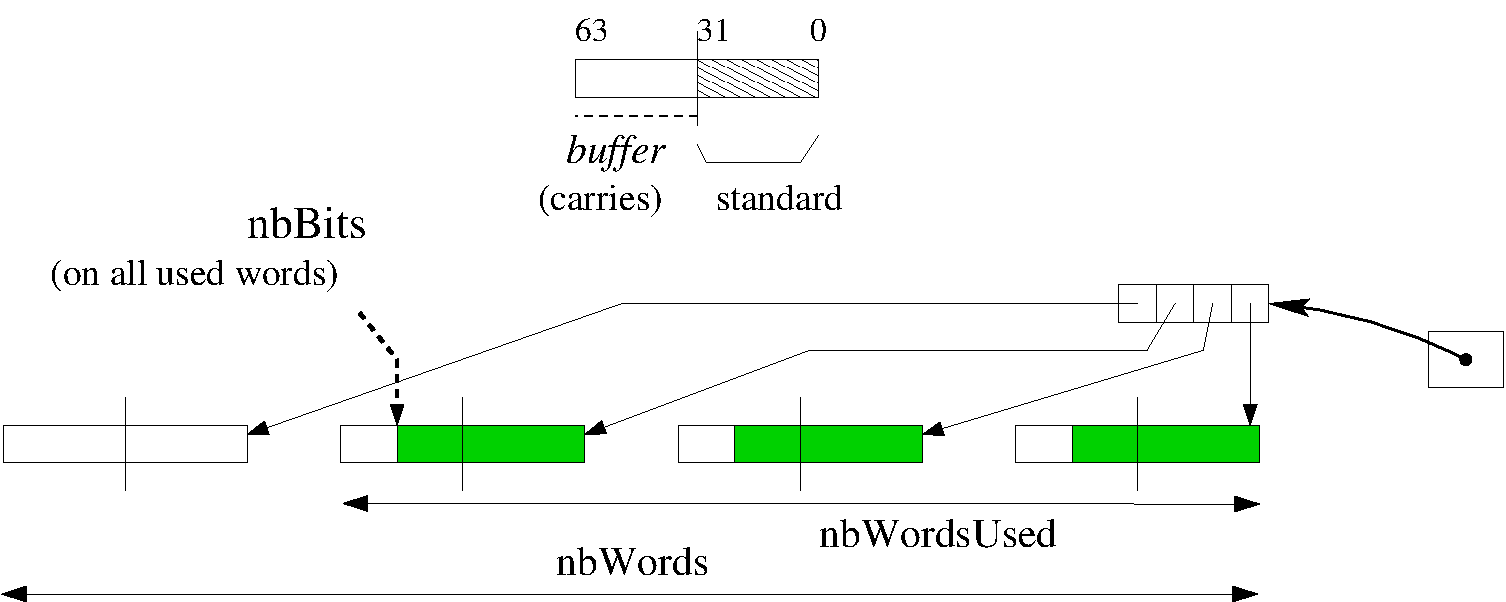
\includegraphics[scale=.5]{\locpath/figures/langford/lgf_grands_entiers}
\caption{Big integer representation, 64 bits words}
\label{fig:big-integer}
\end{figure}
Figure~\ref{fig:big-integer} represents this big integer handling.

This big integer library imposes many constraint on the accelerator memory. 
We conduct tests using simple and double precision for the basic unit. 
The carries propagation is also triggered when necessary only. 
This strategy implies random memory accesses to the words and irregular behavior between the threads. 

\subsubsection{Gray sequence in memory: }
The Gray sequence cannot be stored in an array because it would be too large (it would contain $2^{2n}$ byte values). This is the reason why only one part of the Gray code sequence is stored in memory and the missing terms are directly computed from the known ones using arithmetic considerations.
The size of the stored part of the Gray code sequence is chosen to be as large as possible to be contained in the processor's cache memory, the L1 cache for the GPUs threads: so the accesses are fastened and the computation of the Gray code is optimized.
For an efficient use of the E5-2650 v2 ROMEO's CPUs, which disposes of 20 MB of level-3 cache, the CPU Gray code sequence is developed recursively up to depth 25. For the K20Xm ROMEO's GPUs, which dispose of 8 KB of constant memory, the sequence is developed up to depth 15. The rest of the memory is used for the computation itself. 
%As the Gray sequence is not entirely stored in memory, 
%As we show, all the gray sequence is not in memory, in order to compute the next value when the array is exceeded a modulus method is used for recompute the next value.

\subsubsection{Tasks generation and computation: }
\label{sec:tasks}

In order to perform the computation of the polynomial, two variables can be set among the $2n$ available. For the tasks generation we choose a number $p$ of variables to generate $2^p$ tasks by developing the evaluation tree to depth $p$.\\
 
 
The tasks are spread over the cluster, either synchronously or asynchronously.

\paragraph{Synchronous computation: }
A first experiment was carried out with an MPI distribution of the tasks of the previous model. 
Each MPI process finds its tasks list based on its process \textit{id}; then converting each task number into binary gives the task's initialization. 
The processes work independently; finally the root process ($id=0$) gathers all the computed numbers of solutions and sums them.

\paragraph{Asynchronous computation: }
\label{section:asynchronous}
In this case the tasks can be computed independently. 
As with the synchronous computation, the tasks' initializations are retrieved from their number. 
Each machine can get a task,  compute it, and then store its result; then when all the tasks have been computed, the partial sums are added together and the total result is provided. 

%In this case if a task is cancel due to machine error or another problem, it can be restart without compromising the end of execution.

%\subsubsection{Efficient computation}
%The computation of any task can be summarized in the four following steps:
%\begin{itemize}
%\item First it is necessary to initialize the task: with depth level $p$, $X_1=X_2=1$ and the next $p$ variables are assigned to $1$ or $-1$ depending on the task's id. The following ones are set to $1$ for example.
%\item Secondly it is necessary to set the value of each $S_i$ with the sum of $X_kX_{k + i + 1}$.
%\item Then CPU and GPU, concurrently working, go through all of the Gray sequence on the remaining $2n-p-2$ variables, by updating the $S_i$ and sum their product at each step.
%\item Finally the CPU cores computed results are summed over a shared variable; the GPU sub-tasks results are copied back and then summed with the global result.
%\end{itemize}

\subsection{Experimental settings}
This part presents the experimental context and methodology, and the way the experiments were carried out.
This study has similar goals as for the Miller's resolution experiments.

\subsubsection{Methodology: }
We present here the way the experimental settings were chosen.
Firstly we define the tasks distribution, secondly we set the number of threads per GPU block; finally, we set the CPU/GPU distribution.

\paragraph{Tasks distribution depth: }
This value being set it is important to get a high number of blocks to maintain sufficient GPU load.
Thus we have to determine the best number of tasks for the distribution. As presented in part \ref{sec:tasks} the number $p$ of bits determines $2^p$ tasks. On the one hand, too many tasks are a limitation for the GPU that cannot store all the tasks in its 6GB memory. On the other hand, not enough tasks means longer tasks and too few blocks to fill the GPU grid. figure~\ref{fig:graphe_prof} shows that for the $L(2,23)$ instance the best task number is with generation depth 28.

\paragraph{Number of threads per block: }
In order to take advantage of the GPU computation power, we have to determine the threads/block distribution. Inspired by our experiments with Miller's algorithm we know that the best value may appear at lower occupancy. We perform tests on a given tasks set varying the threads/block number and grid size associated. 
Figure~\ref{fig:graphe_threads} presents the tests performed on the $n=20$ problem: the best distribution is around $128$ threads per block. 
\begin{figure}[t!]
\centering 
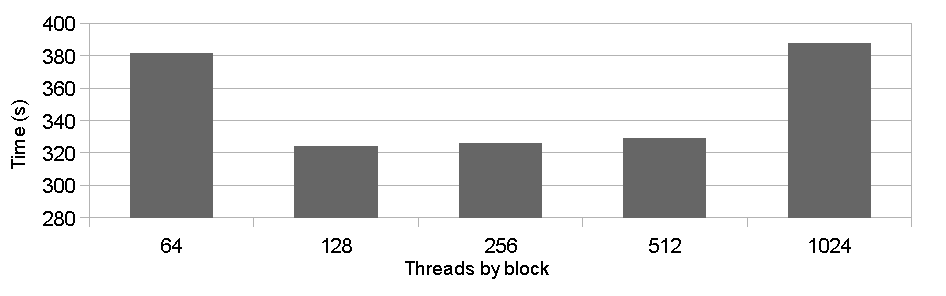
\includegraphics[scale=.55]{\locpath/figures/langford/graphe_threads}
\caption{$L(2,20)$, number of threads per block}
\label{fig:graphe_threads}
\end{figure}

\begin{figure}[t!]
\begin{subfigure}[b]{0.5\linewidth}
\centering 
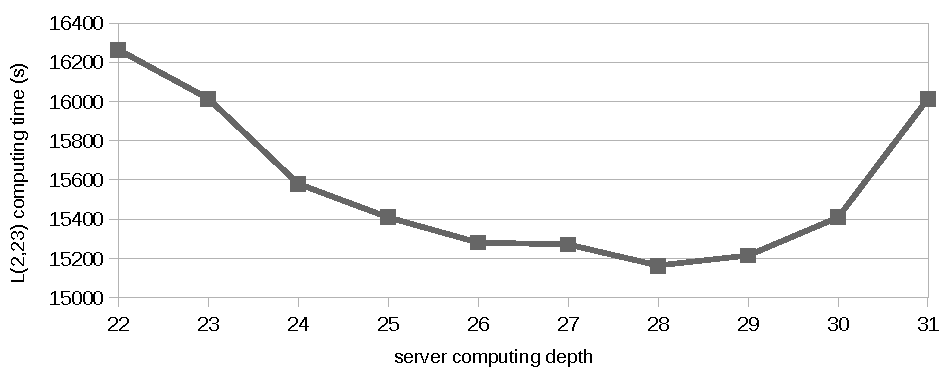
\includegraphics[scale=.5]{\locpath/figures/langford/graphe_prof}
\caption{Influence on server generation depth}
\label{fig:graphe_prof}
\end{subfigure}
\begin{subfigure}[b]{0.5\linewidth}
\centering
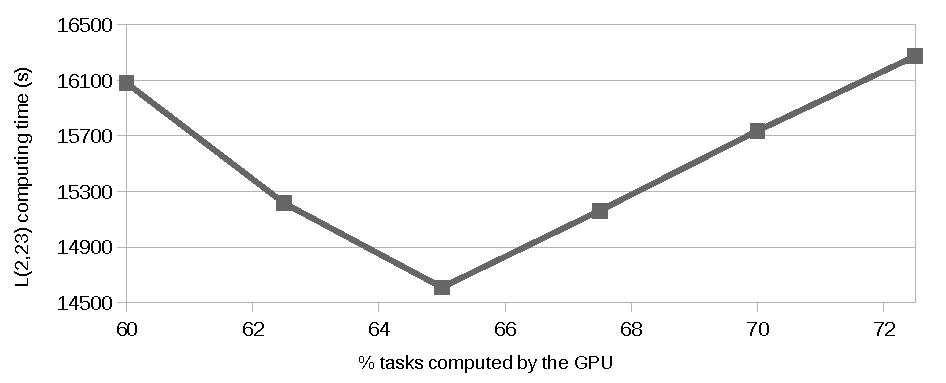
\includegraphics[scale=.5]{\locpath/figures/langford/graphe_cpu_gpu}
\caption{Influence of tasks repartition}
\label{fig:graphe_rep}
\end{subfigure}
\caption{Influences of repartitions of depths and CPU-GPU tasks}
\end{figure}

\subsubsection{CPU vs GPU distribution: }
The GPU and CPU computation algorithm will approximately be the same. 
In order to take advantage of all the computational power of both components we have to balance tasks between CPU and GPU. 
We performed tests by changing the CPU/GPU distribution based on simulations on a chosen set of tasks.  
Figure~\ref{fig:graphe_rep} shows that the best distribution is obtained when the GPU handles 65\% of the tasks. 
This optimal load repartition directly results from the intrinsics computational power of each component; this repartition should be adapted if using a more powerful GPU like Tesla K40 or K80.

\subsubsection{Computing context: }

As presented in part~\ref{sec:part1_ROMEO}, we used the ROMEO supercomputer to perform our tests and computations.
%We use the same supercomputer to perform that computation that we use for the Miller method (section \ref{sec:context}), the ROMEO cluster which use Slurm as node reservation software.
On this supercomputer SLURM\cite{slurm} is used as a reservation and job queue manager.
This software allows two reservation modes: a static one-job limited reservation or the opportunity to dynamically submit several jobs in a Best-Effort manner.

\paragraph{Static distribution: }
In this case we used the synchronous distribution presented in \ref{section:asynchronous}. 
We submited a reservation with the number of MPI processes and the number of cores per process.
This method is useful to get the results quickly if we can get at once a large amount of computation resources. It was used to perform the computation of small problems, and even for $L(2,23)$ and $L(2,24)$.\\
As an issue, it has to be noted that it is difficult to quickly obtain a very large reservation on such a shared cluster, since many projects are currently running. 

\paragraph{Best effort: }
SLURM allows to submit tasks in the specific Best-Effort queue, which does not count in the user \textit{fair-share}. In this queue, if a node is free and nobody is using it, the reservation is set for a job in the best effort queue for a minimum time reservation. 
If another user asks for a reservation and requests this node, the best effort job is killed (with, for example, a SIGTERM signal). This method, based on asynchronous computation, enables a maximal use of the computational resources without blocking for a long time the entire cluster.
%This global computation process is fault-tolerant since no result is provided for aborted tasks, that are computed again.

For $L(2,27)$ and even more for $L(2,28)$ the total time required is too important to use the whole machine off a challenge period, thus we chose to compute in a Best-Effort manner.
In order to fit with this submission method we chose a reasonable time-per-task, sufficient to optimize the treatments with low loading overhead, but not too long so that killed tasks are not too penalizing for the global computation time. We empirically chose to run 15-20 minute tasks and thus we considered $p=15$ for $n=27$ and $p=17$ for $n=28$. 

The best effort based algorithm is presented on figure~\ref{fig:graphe_besteffort}.
The task handler maintains a maximum of 256 tasks in the queue; in addition the entire process is designed to be fault-tolerant since killed tasks have to be launched again.
When finished, the tasks generate an output containing the number of solutions and computation time, that is stored as a file or database entry. 
At the end the outputs of the different tasks are merged and the global result can be provided.  

\begin{figure}[t!]
\centering
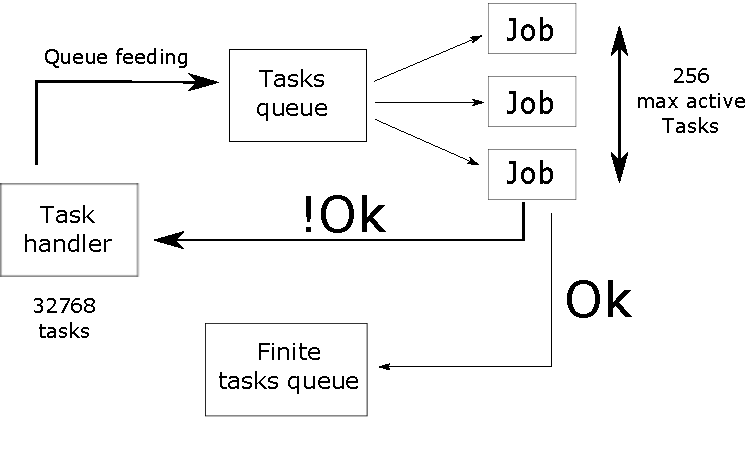
\includegraphics[scale=.6]{\locpath/figures/langford/best_effort}
\caption{Best-effort distribution}
\label{fig:graphe_besteffort}
\end{figure}

%\begin{algorithm}[htbp]
%\caption{Server distribution}
%\begin{algorithmic} 
%\STATE \textbf{Variables :}
%\STATE $TQ$: tasks queue, task = integer
%\STATE $FQ$: finished tasks queue, task = integer
%\STATE $BEQ$: number of elements in the Best-Effort queue
%\STATE $N$: number of tasks
%\STATE $result$: final result
%\STATE $nbMachines$: Best-Effort queue jobs limitation
%\STATE 
%\STATE \textbf{Begin}
%\STATE $TQ\leftarrow$generate\_tasks($N$)
%\WHILE{$\#FQ \neq N$}
%\IF{$BEQ < nbMachines$}
%\STATE Start($TQ.next$)
%\ENDIF
%\ENDWHILE
%\STATE $result\leftarrow$sum($FQ$)
%\STATE \textbf{End}
%\end{algorithmic}
%\label{algo:server}
%\end{algorithm}
%
%\begin{algorithm}[htbp]
%\caption{Client task handling}
%\begin{algorithmic}
%\STATE \textbf{Variables :}
%\STATE $TQ$: tasks queue, task = integer
%\STATE $FQ$: finished tasks queue, task = integer
%\STATE $n$: number of this task
%\STATE 
%\STATE \textbf{Signal handler :}
%\IF{$SIGKILL$}
%\STATE put $n$ in the $TQ$
%\ENDIF
%\STATE 
%\STATE \textbf{Begin}
%\STATE $solution\leftarrow$compute($N$)
%\IF{$Error$}
%\STATE put $n$ in $TQ$
%\ELSE
%\STATE put $solution$ in $FQ$
%\ENDIF
%\STATE \textbf{End}
%\end{algorithmic}
%\label{algo:client}
%\end{algorithm}

\subsection{Results}
After these optimizations and implementation tuning steps, we conducted tests on the ROMEO supercomputer using best-effort queue to solve $L(2,27)$ and $L(2,28)$. 
We started the experiment after an update of the supercomputer, that implied a cluster shutdown. 
Then the machine was restarted and was about 50\% idle for the duration of our challenge. 
The computation lasted less than 2 days for $L(2,27)$ and 23 days for $L(2,28)$. 
The following describes performances considerations.

\textbf{Computing effort -} 
For $L(2,27)$, the effective computation time of the 32,768 tasks was about 30 million seconds (345.4 days), and 165,000" elapsed time (1.9 days); the average time of the tasks was 911", with a standard deviation of 20\%.
For the $L(2,28)$ 131,072 tasks the total computation time was about 1365 days (117 million seconds), as 23 day elapsed time; the tasks lasted 1321" on average with a 12\% standard deviation.

\textbf{Best-effort overhead -} 
With $L(2,27)$ we used a specific database to maintain information concerning the tasks: 617 tasks were aborted [by regular user jobs] before finishing (1.9\%), with an average computing time of 766" (43\% of the maximum requested time for a task). This consumed 472873", which overhead represents 1.6\% of the effective computing effort.

\textbf{Cluster occupancy -}
Figure~\ref{fig:graphe_15minutes_27} presents the tasks resolution over the two computation days for $L(2,27)$.
The experiment elapse time was 164700" (1.9 days). Compared to the effective computation time, we used an average of 181.2 machines (CPU-GPU couples): this represents 69.7\% of the entire cluster.
 
Figure~\ref{fig:graphe_15minutes_28} presents the tasks resolution flow during the 23 days computation for $L(2,28)$. We used about 99 machines, which represents 38\% of the 230 available nodes.

\begin{figure}[t!]
\begin{subfigure}[b]{0.5\linewidth}
\centering
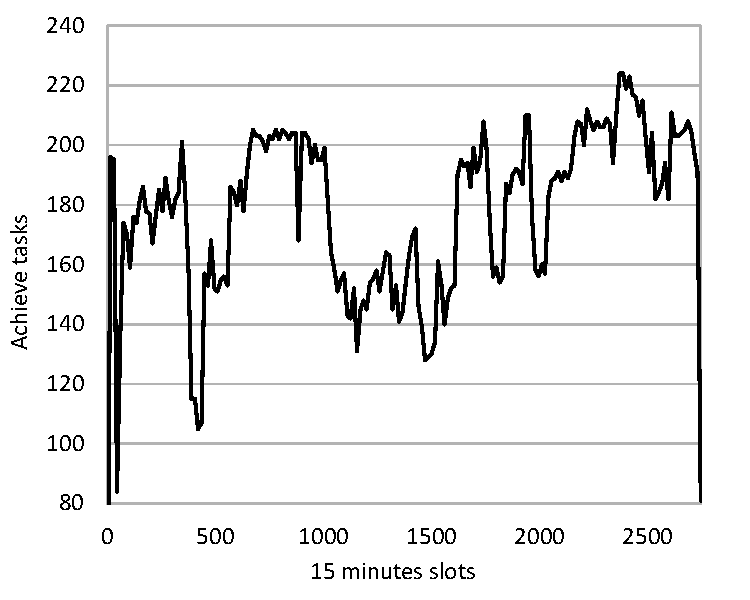
\includegraphics[scale=.6]{\locpath/figures/langford/graphe_15minutes_petit}
\caption{$L(2,27)$ tasks grouped by 15" slots}
\label{fig:graphe_15minutes_27}
\end{subfigure}
\begin{subfigure}[b]{0.5\linewidth}
\centering
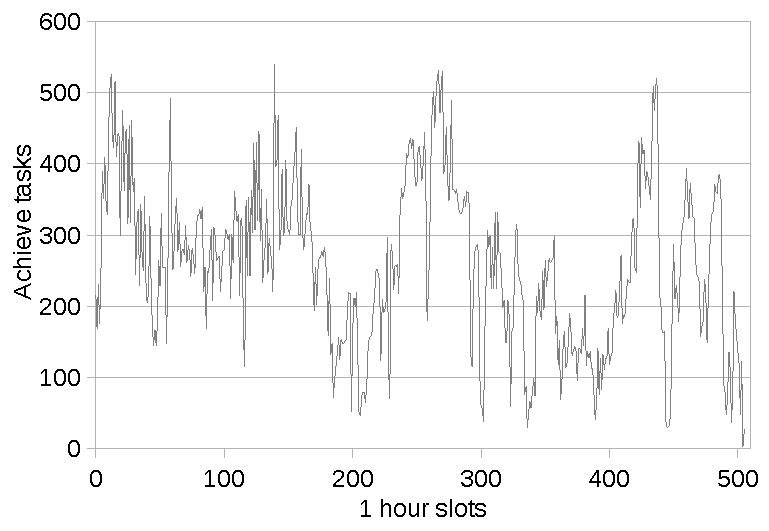
\includegraphics[scale=.6]{\locpath/figures/langford/graphe_15minutes_petit_28}
\caption{$L(2,28)$ tasks grouped by 1 hour slots}
\label{fig:graphe_15minutes_28}
\end{subfigure}
\caption{Task repartition for $L(2,27)$ and $L(2,28)$ }
\end{figure}

For $L(2,27)$, these results confirm that the computation took great advantage of the low occupancy of the cluster during the experiment. 
This allowed us to obtain a weak best-effort overhead, and an important cluster occupancy. 
Unfortunately for $L(2,28)$ on such a long period we got a lower part of the supercomputer dedicated to our computational project.
Thus we are confident in good perspectives for the $L(2,31)$ instance if computed on an even larger cluster or several distributed clusters. 

\section{Conclusion}
%\todo{Refaire la conclusion pour mettre en avant les resultats}

This first benchmark presents two methods to solve the Langford pairing problem on multi-GPU clusters. 
Those methods are presented as the Miller's and Godfrey's algorithms.

\subsection{Miller's method: irregular memory + computation}
In this first implementation we showed that the accelerator can target irregularity in memory and computation. 
The tree traversal, even with branch cutting, gives us excellent results on many-core architecture.
They GPUs handle 80\% of the computation effort.
Also as any combinatorial problem can be represented as a CSP, the Miller algorithm can be seen as general resolution scheme based on the backtrack tree browsing. 
A three-level tasks generation allows to fit the multiGPU architecture. 
MPI or Best-Effort are used to spread tasks over the cluster, OpenMP for the CPU cores distribution and then CUDA to take advantage of the GPU computation power.
We were able to compute $L(2,20)$ with this regularized method and to get an even better time with the basic backtrack. 
This proves the proposed approach and also exhibits that the GPU scheduler is very efficient at managing highly divergent threads.

\subsection{Godfrey's method: irregular memory + heavy computation}
We also presented the Godfrey's method which target irregular memory accesses but also heavy computational behavior. 
The results shows that the many-core version completely exceed the classical processor best performances. 
The GPU handle 65\% of the computation effort. 
In addition we beat the Langford limits using multi-GPUs. 
In order to use the supercomputer ROMEO, which is shared by a large scientific community, we have implemented a distribution that does not affect the machine load, using a best-effort queue. The computation is fault-tolerant and totally asynchronous.
The utilization of this technology also show the reliability of nowadays accelerators technologies. 
Indeed, they can be use at demand on specific tasks without specific warm-up. 

\paragraph{Langford problem results: }
This work also enabled us to compute $L(2,27)$ and $L(2,28)$ in respectively less than 2 days and 23 days on the University of Reims ROMEO supercomputer. 
This is the fastest time on those problems nowadays.
The total number of solutions is: 

\hspace{3cm} L(2,27) = 111,683,611,098,764,903,232

\hspace{3cm} L(2,28) = 1,607,383,260,609,382,393,152\\

This first benchmark implementation is clearly in favor of hybrid architecture. 
The many-core architecture shows a perfect handling of irregularity and heavy computations. 
